% "Where to move from S?" Adapted from the CAEPIA 2026 slides.
\documentclass[border=0pt]{standalone}
% Shared preamble of the GSO-RL documentation figures.
% Compiled with latex (DVI) + dvisvgm; see ../build.sh.
\def\pgfsysdriver{pgfsys-dvisvgm.def}
\usepackage[T1]{fontenc}
\usepackage{lmodern}
\renewcommand{\familydefault}{\sfdefault}
\usepackage{amsmath, amssymb}
\usepackage{tikz}
\usetikzlibrary{positioning, shapes, arrows.meta, calc, fit, backgrounds}

% Palette
\definecolor{Purple}{RGB}{102, 0, 153}
\colorlet{ColMa}{green!50!black}   % macro-move M1
\colorlet{ColMb}{blue!70!black}    % macro-move M2
\colorlet{ColMc}{orange!85!black}  % macro-move M3
\definecolor{cGa}{RGB}{38, 166, 154}
\definecolor{cGb}{RGB}{229, 96, 76}
\definecolor{cGc}{RGB}{235, 165, 40}
\definecolor{cGd}{RGB}{125, 125, 215}
\definecolor{cGe}{RGB}{190, 60, 150}

% White background so figures stay readable in dark mode. The white rectangle lives on the
% "background" layer; figures draw their own backdrops on "behind", which sits above it.
\pgfdeclarelayer{behind}
\pgfsetlayers{background,behind,main}
\tikzset{every picture/.append style={show background rectangle,
  background rectangle/.style={fill=white, draw=none}, inner frame sep=8pt}}
% NOTE: with dvisvgm, text placed after a \color{...} group inside the same node is misplaced.
% Put differently coloured pieces of text in separate nodes.

\newcommand{\yes}{{\color{green!50!black}\checkmark}}
\newcommand{\nope}{{\color{red!70!black}$\boldsymbol{\times}$}}

% A region: guide with three concentric rings.  \guia[style]{x}{y}{color}{label}
\newcommand{\guia}[5][]{%
  \fill[#4!10, #1] (#2,#3) circle (1.05);
  \fill[#4!20, #1] (#2,#3) circle (0.7);
  \fill[#4!35, #1] (#2,#3) circle (0.35);
  \foreach \r in {0.35,0.7,1.05} \draw[#4, #1] (#2,#3) circle (\r);
  \fill[#4!80!black, #1] (#2,#3) circle (2pt);
  \node[#4!75!black, font=\scriptsize\bfseries, #1] at (#2,#3+1.22) {#5};
}

\begin{document}
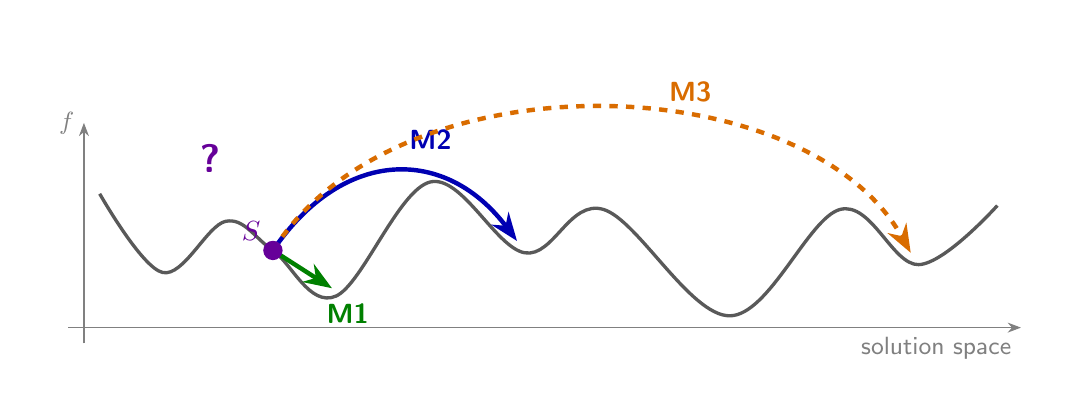
\begin{tikzpicture}[>=Stealth]
  \draw[->, gray] (-0.2,0) -- (11.9,0) node[below left, font=\small] {solution space};
  \draw[->, gray] (0,-0.2) -- (0,2.6) node[left, font=\small] {$f$};
  \draw[very thick, gray!70!black] plot[smooth, tension=0.6] coordinates {
    (0.2,1.7) (1,0.7) (1.8,1.35) (2.4,0.98) (3.2,0.4) (4.4,1.85) (5.6,0.95)
    (6.6,1.5) (8.2,0.15) (9.6,1.5) (10.6,0.8) (11.6,1.55)};
  \coordinate (S) at (2.4,0.98);
  \draw[->, ultra thick, ColMa] (S) -- (3.15,0.5);
  \node[ColMa, font=\bfseries, anchor=north] at (3.35,0.42) {M1};
  \draw[->, ultra thick, ColMb] (S) .. controls (3.3,2.3) and (4.6,2.3) .. (5.5,1.1);
  \node[ColMb, font=\bfseries] at (4.4,2.38) {M2};
  \draw[->, ultra thick, ColMc, dashed] (S) .. controls (4,3.5) and (9.2,3.3) .. (10.5,0.95);
  \node[ColMc, font=\bfseries] at (7.7,3.0) {M3};
  \fill[Purple] (S) circle (3.5pt);
  \node[above left=0pt and 1pt of S, font=\bfseries, Purple] {$S$};
  \node[font=\Large\bfseries, Purple] at (1.6,2.15) {?};
\end{tikzpicture}
\end{document}
